\chapter{Data Splitting and Generalization}
\label{chap:data_splitting}

% ========================================
% SECTION 1: THE GOAL OF ML
% ========================================
\section{The Cardinal Rule of Machine Learning}
Imagine a student preparing for an exam.
\begin{itemize}
    \item \textbf{Scenario A}: The student memorizes the answers to the practice questions perfectly.
    \item \textbf{Scenario B}: The student understands the concepts and can solve \textit{new} questions they have never seen before.
\end{itemize}

In Machine Learning, we want Scenario B.
\begin{definition}
\textbf{Generalization}: The ability of a model to perform well on \textbf{unseen data} (data it did not see during training).
\end{definition}

If a model memorizes the training data (Scenario A), it has failed, even if it scores 100\% accuracy on that data. This is called \textbf{Overfitting}.

% ========================================
% SECTION 2: WHY WE SPLIT
% ========================================
\section{The Train-Test Split}
To ensure our model generalizes, we must hide some data from it during training. We treat this hidden data as a "Mock Exam".

\begin{figure}[htbp]
\centering
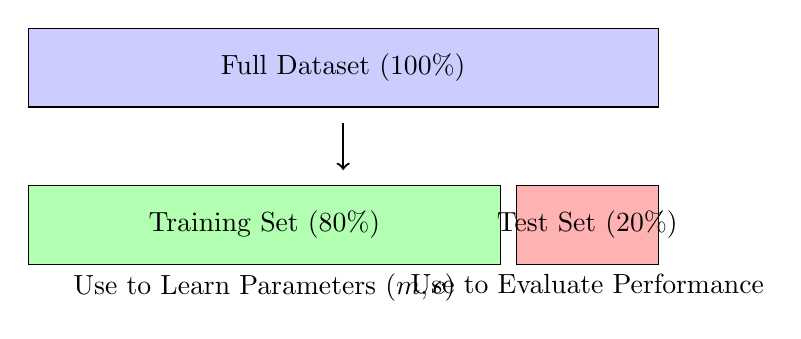
\begin{tikzpicture}
    \draw[fill=blue!20] (0,0) rectangle (8,1);
    \node at (4, 0.5) {Full Dataset (100\%)};
    
    \draw[->, thick] (4, -0.2) -- (4, -0.8);
    
    \draw[fill=green!30] (0,-2) rectangle (6,-1);
    \node at (3, -1.5) {Training Set (80\%)};
    \node[below] at (3, -2) {Use to Learn Parameters ($m, c$)};
    
    \draw[fill=red!30] (6.2,-2) rectangle (8,-1);
    \node at (7.1, -1.5) {Test Set (20\%)};
    \node[below] at (7.1, -2) {Use to Evaluate Performance};
\end{tikzpicture}
\caption{The Train-Test Split allows us to estimate real-world performance.}
\label{fig:train_test_split}
\end{figure}

\begin{enumerate}
    \item \textbf{Training Set}: Used to fit the model (calculate gradients, update weights). The model \textit{sees} labels here.
    \item \textbf{Test Set}: Used \textbf{ONLY} for evaluation. The model \textit{never} sees these labels during training.
\end{enumerate}

\begin{quote}
\textbf{Golden Rule}: Never train on your Test Set. This is \textbf{Data Leakage}, and it is a cheating sin.
\end{quote}

% ========================================
% SECTION 3: THE VALIDATION SET
% ========================================
\section{Going Deeper: The Validation Set}
What if we want to tune hyperparameters (like $K$ in KNN, or $\lambda$ in Ridge)?
\begin{itemize}
    \item If we tune $K$ to maximize Test Accuracy, we are indirectly "peeking" at the Test Set. The Test Set is no longer "Unseen".
\end{itemize}

\textbf{Solution}: The 3-way Split.
\begin{enumerate}
    \item \textbf{Train}: Learn parameters.
    \item \textbf{Validation (Dev)}: Tune hyperparameters.
    \item \textbf{Test}: Final honest evaluation.
\end{enumerate}

% ========================================
% SECTION 4: CROSS VALIDATION
% ========================================
\section{K-Fold Cross-Validation}
If we have a small dataset, splitting 20\% for testing might leave us with very little training data. Also, maybe that specific 20\% was just "lucky" or "hard".

\textbf{Solution}: K-Fold Cross-Validation.
\begin{enumerate}
    \item Divide data into $K$ equal parts (Average $K=5$ or $10$).
    \item Train on $K-1$ parts, Test on the remaining 1 part.
    \item Repeat $K$ times, rotating the Test part.
    \item Average the scores.
\end{enumerate}

This gives a much more robust estimate of model performance.

% ========================================
% SECTION 5: IMPLEMENTATION
% ========================================
\section{Implementation in Python}
\begin{lstlisting}[language=Python, caption=Train-Test Split]
from sklearn.model_selection import train_test_split

# X: Features, y: Target
# test_size=0.2 means 20% data goes to Test Set
# random_state=42 ensures the split is the same every time we run
X_train, X_test, y_train, y_test = train_test_split(
    X, y, test_size=0.2, random_state=42
)

print(f"Training Shape: {X_train.shape}")
print(f"Testing Shape: {X_test.shape}")

# Train ONLY on X_train
model.fit(X_train, y_train)

# Evaluate on X_test
score = model.score(X_test, y_test)
\end{lstlisting}

% ========================================
% SECTION 6: HOTS QUESTIONS
% ========================================
\section{HOTS: Interview Questions}
\textbf{Q1: What happens if you train on your Test Data?}
\begin{itemize}
    \item This is \textbf{Model Overfitting/Data Leakage}. Usually you get amazing accuracy (e.g. 99\%) in the lab, but the model fails drastically in production.
\end{itemize}

\textbf{Q2: Is a random split always good?}
\begin{itemize}
    \item Not always. For \textbf{Time Series} data (Stock prices), you cannot split randomly. You must split by time (Train: Jan-Oct, Test: Nov-Dec).
    \item For \textbf{Imbalanced Data}, you should use \textbf{Stratified Split} to ensure the class ratio is preserved in both sets.
\end{itemize}

% ========================================
% SECTION 7: QUICK REFERENCE
% ========================================
\section{Quick Reference Card}

\begin{center}
\fbox{\parbox{0.9\textwidth}{
\textbf{DATA SPLITTING - CHEAT SHEET}
\vspace{0.3cm}

\textbf{Golden Rule}: Never fit/train on Test Data. Test Data is for Final Exam only.

\textbf{Standard Splits}:
\begin{itemize}
    \item \textbf{Simple}: 80\% Train, 20\% Test (for large data).
    \item \textbf{3-Way}: 60\% Train $\rightarrow$ 20\% Val (Tune) $\rightarrow$ 20\% Test (Evaluate).
\end{itemize}

\textbf{Techniques}:
\begin{center}
\begin{tabular}{|l|l|}
\hline
\textbf{Scenario} & \textbf{Method} \\ \hline
Standard & Random Split \\ \hline
Small Dataset & K-Fold Cross Validation \\ \hline
Imbalanced & Stratified Split (keeps ratios) \\ \hline
Time Series & Time-based Split (No shuffle!) \\ \hline
\end{tabular}
\end{center}

\textbf{Sklearn}:
\begin{itemize}
    \item \texttt{train\_test\_split(X, y, test\_size=0.2, stratify=y)}
    \item \texttt{cross\_val\_score(model, X, y, cv=5)}
\end{itemize}

\textbf{Interview Gold}:
\begin{itemize}
    \item Validation Set is for Tuning (Hyperparameters).
    \item Test Set is for Reporting (Generalization Error).
    \item Data Leakage = optimizing on Test Set = Cheating.
\end{itemize}
}}
\end{center}
